% ------------------------------------------------------------------------
% ------------------------------------------------------------------------
% abnTeX2: Modelo de Trabalho Academico (tese de doutorado, dissertacao de
% mestrado e trabalhos monograficos em geral) em conformidade com
% ABNT NBR 14724:2011: Informacao e documentacao - Trabalhos academicos -
% Apresentacao
% ------------------------------------------------------------------------
% ------------------------------------------------------------------------

\documentclass[
	% -- opções da classe memoir --
	12pt,				% tamanho da fonte
	openright,			% capítulos começam em pág ímpar (insere página vazia caso preciso)
	twoside,			% para impressão em recto e verso. Oposto a oneside
	a4paper,			% tamanho do papel.
	% -- opções da classe abntex2 --
	%chapter=TITLE,		% títulos de capítulos convertidos em letras maiúsculas
	%section=TITLE,		% títulos de seções convertidos em letras maiúsculas
	%subsection=TITLE,	% títulos de subseções convertidos em letras maiúsculas
	%subsubsection=TITLE,% títulos de subsubseções convertidos em letras maiúsculas
	% -- opções do pacote babel --
	english,			% idioma adicional para hifenização
	brazil,				% o último idioma é o principal do documento
	svgnames
	]{abntex2}\usepackage[]{graphicx}\usepackage[]{color}
% maxwidth is the original width if it is less than linewidth
% otherwise use linewidth (to make sure the graphics do not exceed the margin)
\makeatletter
\def\maxwidth{ %
  \ifdim\Gin@nat@width>\linewidth
    \linewidth
  \else
    \Gin@nat@width
  \fi
}
\makeatother

\definecolor{fgcolor}{rgb}{0.345, 0.345, 0.345}
\newcommand{\hlnum}[1]{\textcolor[rgb]{0.686,0.059,0.569}{#1}}%
\newcommand{\hlstr}[1]{\textcolor[rgb]{0.192,0.494,0.8}{#1}}%
\newcommand{\hlcom}[1]{\textcolor[rgb]{0.678,0.584,0.686}{\textit{#1}}}%
\newcommand{\hlopt}[1]{\textcolor[rgb]{0,0,0}{#1}}%
\newcommand{\hlstd}[1]{\textcolor[rgb]{0.345,0.345,0.345}{#1}}%
\newcommand{\hlkwa}[1]{\textcolor[rgb]{0.161,0.373,0.58}{\textbf{#1}}}%
\newcommand{\hlkwb}[1]{\textcolor[rgb]{0.69,0.353,0.396}{#1}}%
\newcommand{\hlkwc}[1]{\textcolor[rgb]{0.333,0.667,0.333}{#1}}%
\newcommand{\hlkwd}[1]{\textcolor[rgb]{0.737,0.353,0.396}{\textbf{#1}}}%
\let\hlipl\hlkwb

\usepackage{framed}
\makeatletter
\newenvironment{kframe}{%
 \def\at@end@of@kframe{}%
 \ifinner\ifhmode%
  \def\at@end@of@kframe{\end{minipage}}%
  \begin{minipage}{\columnwidth}%
 \fi\fi%
 \def\FrameCommand##1{\hskip\@totalleftmargin \hskip-\fboxsep
 \colorbox{shadecolor}{##1}\hskip-\fboxsep
     % There is no \\@totalrightmargin, so:
     \hskip-\linewidth \hskip-\@totalleftmargin \hskip\columnwidth}%
 \MakeFramed {\advance\hsize-\width
   \@totalleftmargin\z@ \linewidth\hsize
   \@setminipage}}%
 {\par\unskip\endMakeFramed%
 \at@end@of@kframe}
\makeatother

\definecolor{shadecolor}{rgb}{.97, .97, .97}
\definecolor{messagecolor}{rgb}{0, 0, 0}
\definecolor{warningcolor}{rgb}{1, 0, 1}
\definecolor{errorcolor}{rgb}{1, 0, 0}
\newenvironment{knitrout}{}{} % an empty environment to be redefined in TeX

\usepackage{alltt}

% ---
% Novo list of (listings) para QUADROS
% ---

%\newcommand{\quadroname}{Quadro}
%\newcommand{\listofquadrosname}{Lista de quadros}

%\newfloat[chapter]{quadro}{loq}{\quadroname}
%\newlistof{listofquadros}{loq}{\listofquadrosname}
%\newlistentry{quadro}{loq}{0}

% configurações para atender às regras da ABNT
%\counterwithout{quadro}{chapter}
%\renewcommand{\cftquadroname}{\quadroname\space}
%\renewcommand*{\cftquadroaftersnum}{\hfill--\hfill}

% ---
% PACOTES
% ---
\usepackage{lscape}
% ---
% Pacotes fundamentais
% ---
\usepackage{lmodern}			% Usa a fonte Latin Modern
\usepackage[T1]{fontenc}		% Selecao de codigos de fonte.
\usepackage[utf8]{inputenc}		% Codificacao do documento (conversão automática dos acentos)
\usepackage{indentfirst}		% Indenta o primeiro parágrafo de cada seção.
\usepackage{color}			% Controle das cores
\usepackage{graphicx}			% Inclusão de gráficos
\usepackage{microtype} 			% para melhorias de justificação
\usepackage{setspace}
\usepackage{wrapfig}

% ---
% Para titulo em destaque sem sequencia de numeração
% ---
\newcommand{\datatitle}[1]{
  \normalsize \textsc{#1}
}

% ---
% Funções matematicas
% ---
\usepackage{amsmath,amssymb,amstext}
\usepackage{mathtools}                  % Funcionalidades (como \dcases)
\usepackage{dsfont}    %% Para \mathds{1} Indicadora
\usepackage{bm}

\DeclareMathOperator{\Ell}{\mathcal{L}}
\DeclareMathOperator{\R}{\mathbb{R}}
\DeclareMathOperator{\ind}{\mathds{1}}

\DeclareRobustCommand{\rchi}{{\mathpalette\irchi\relax}}
\newcommand{\irchi}[2]{\raisebox{\depth}{$#1\chi$}}

% ---
% Para tabelas
% ---
\usepackage{multirow}
\usepackage{array}
\usepackage{threeparttable}

% ---
% Pacotes e definições adcionais, para adequações especificas
% ---
\usepackage{tikz}
\usepackage{pdflscape}			% para ambiente landscape
\usepackage{pgfgantt}			% cronograma estilo gráfico de gantt
\usepackage{multicol}
\usetikzlibrary{backgrounds}
\usepackage{tasks}

% ---
% Fontes matemáticas
% ---
\usepackage{mathpazo}
\usepackage{inconsolata}
\usepackage{verbatim}

% ---
% Pacotes adicionais, usados apenas no âmbito do Modelo Canônico do abnteX2
% ---
\usepackage{lipsum}				% para geração de dummy text
% ---

% ---
% Pacotes de citações
% ---
\usepackage[brazilian,hyperpageref]{backref}% Paginas com as citações
\usepackage[alf, abnt-etal-list=0]{abntex2cite}				% Citações padrão ABNT

% ---
% CONFIGURAÇÕES DE PACOTES
% ---

% ---
% Configurações do pacote backref
% Usado sem a opção hyperpageref de backref
\renewcommand{\backrefpagesname}{Citado na(s) página(s):~}
% Texto padrão antes do número das páginas
\renewcommand{\backref}{}
% Define os textos da citação
\renewcommand*{\backrefalt}[4]{
  \ifcase #1 %
  Nenhuma citação no texto.%
  \or
  Citado na página #2.%
  \else
  Citado #1 vezes nas páginas #2.%
  \fi}%
% ---

% ---
% Informações de dados para CAPA e FOLHA DE ROSTO
% ---
\titulo{Aprendizado de máquina \\ Laboratório 1 - Impactos da Representação}
\vspace{2cm}
\autor{Lineu Alberto Cavazani de Freitas}
\local{Curitiba}
\data{2021}
\instituicao{Universidade Federal do Paraná}

\preambulo{Relatório apresentado à disciplina
    Aprendizado de Máquina, ministrada pelo professor Luiz Eduardo Soares de Oliveira, no Programa de Pós Graduação em Informática da Universidade Federal do Paraná.}
% ---

% ---
% Configurações de aparência do PDF final

% informações do PDF
\makeatletter
\hypersetup{
  % pagebackref=true,
  pdftitle={\@title},
  pdfauthor={\@author},
  pdfsubject={\imprimirpreambulo},
  pdfcreator={LaTeX with abnTeX2},
  % pdfkeywords={abnt}{latex}{abntex}{abntex2}{projeto de pesquisa},
  colorlinks=true,	% false: boxed links; true: colored links
  linkcolor=blue,     % color of internal links
  citecolor=blue, % color of links to bibliography
  filecolor=magenta, % color of file links
  urlcolor=black,
  bookmarksdepth=4
}
\addto\captionsbrazil{
  \renewcommand{\bibname}{REFER\^ENCIAS}
}
\makeatother
% ---

% ---
% Espaçamentos entre linhas e parágrafos
% ---

% O tamanho do parágrafo é dado por:
\setlength{\parindent}{1.3cm}

% Controle do espaçamento entre um parágrafo e outro:
\setlength{\parskip}{0.2cm}  % tente também \onelineskip

% ---
% Highlight knitr code (pode-usar usar os varios highligths já definidos
% com thm = knit_theme$get("nuvola"); knit_theme$set(thm))
% ---

\renewcommand{\hlnum}[1]{\textcolor[rgb]{0.733,0,1}{#1}}%
\renewcommand{\hlstr}[1]{\textcolor[rgb]{0,0.533,0}{#1}}%
\renewcommand{\hlcom}[1]{\textcolor[rgb]{0,0,0}{#1}}%
\renewcommand{\hlopt}[1]{\textcolor[rgb]{0.412,0.412,0.412}{#1}}%
\renewcommand{\hlstd}[1]{\textcolor[rgb]{0.2,0.2,0.2}{{#1}}}%
\renewcommand{\hlkwa}[1]{\textcolor[rgb]{0.2,0.2,0.2}{{#1}}}%
\renewcommand{\hlkwb}[1]{\textcolor[rgb]{0.4,0,0}{\textbf{#1}}}%
\renewcommand{\hlkwc}[1]{\textcolor[rgb]{0.13,0.29,0.53}{#1}}%
\renewcommand{\hlkwd}[1]{\textcolor[rgb]{0.13,0.29,0.53}{\textbf{#1}}}%

% ---
% compila o indice
% ---
\makeindex
% ---

% ----
% Início do documento
% ----
\IfFileExists{upquote.sty}{\usepackage{upquote}}{}
\begin{document}

% Seleciona o idioma do documento (conforme pacotes do babel)
% \selectlanguage{english}
\selectlanguage{brazil}

% Retira espaço extra obsoleto entre as frases.
\frenchspacing

% ----------------------------------------------------------
% ELEMENTOS PRÉ-TEXTUAIS
% ----------------------------------------------------------
% \pretextual

% ---
% Capa
% ---
\tikz[remember picture,overlay] \node[opacity=1,inner sep=0pt] at
(current page.center){
  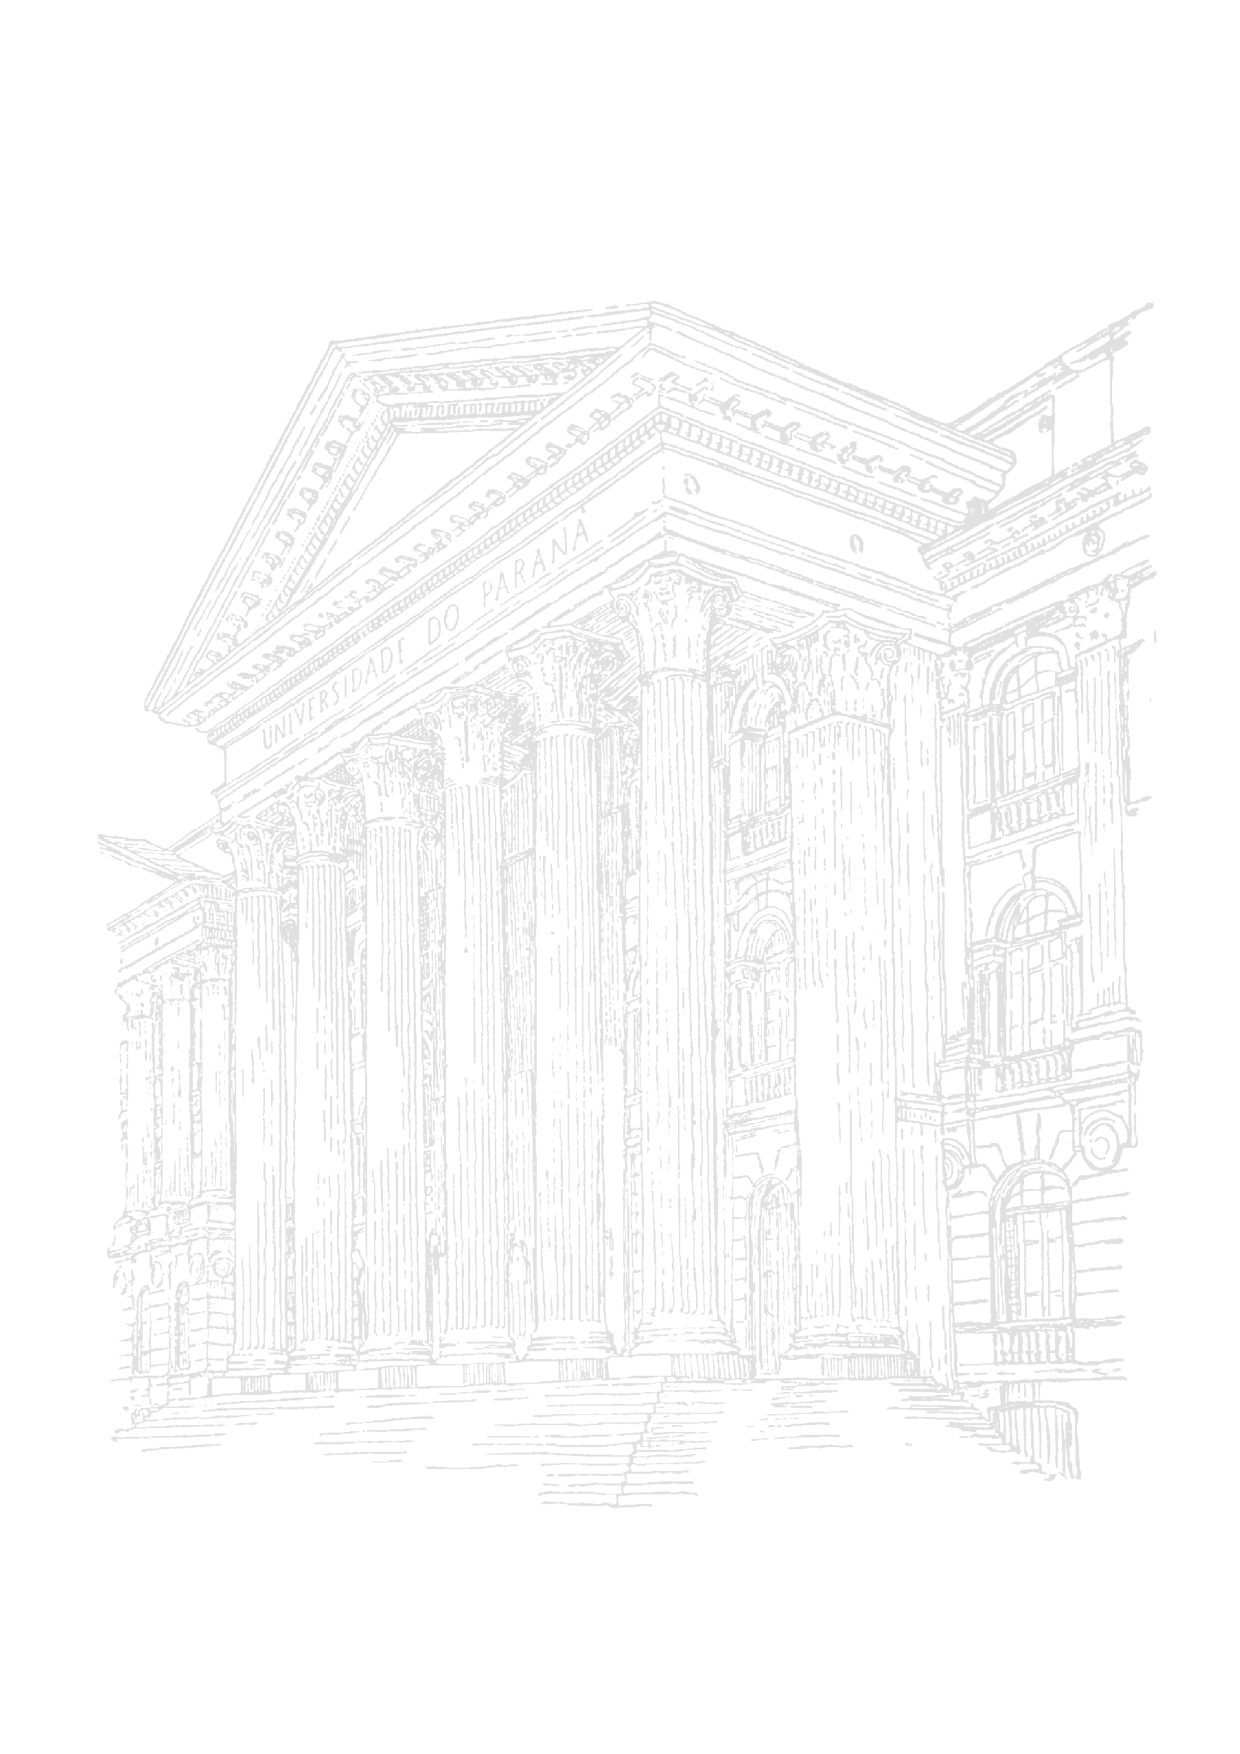
\includegraphics[width=\paperwidth,
  height=\paperheight]{images/ufpr_bg}};

\begin{center}
  {\Large \textsf{Universidade Federal do Paraná}}
  \vspace{-0.5cm}
\end{center}

\imprimircapa

% ---

% ---
% Folha de rosto
% ---
\imprimirfolhaderosto
% ---

% ---
% Dedicatória
% ---
% \begin{dedicatoria}
%   \lipsum[1]
% \end{dedicatoria}
% ---

% ---
% Agradecimentos
% ---
% \begin{agradecimentos}
%   \lipsum[1]
% \end{agradecimentos}
% ---

% ---
% Epígrafe
% ---
%\begin{epigrafe}
%    \vspace*{\fill}
%	\begin{flushright}
%          \textit{``Software is like sex: it's better when \\
%            it's free``}\\
%          --- Linus Torvalds \\[1cm]

%          \textit{``The numbers are where the scientific \\ discussion
%            should start, not end.''}\\
%          --- Steven N. Goodman
%	\end{flushright}
%\end{epigrafe}
% ---

% ---
% RESUMOS
% ---

% resumo em português
%\setlength{\absparsep}{18pt} % ajusta o espaçamento dos parágrafos do resumo
%\begin{resumo}


% ---
% inserir lista de ilustrações
% ---
%\pdfbookmark[0]{\listfigurename}{lof}
%\listoffigures*
%\cleardoublepage
% ---

% ---
% inserir lista de tabelas
% ---
%\pdfbookmark[0]{\listtablename}{lot}
%\listoftables*
%\cleardoublepage
% ---

% ---
% inserir lista de quadros
% ---
%\pdfbookmark[0]{\listofquadrosname}{loq}
%\listofquadros*
%\cleardoublepage
% ---

% ---
% inserir lista de abreviaturas e siglas
% ---
% \begin{siglas}
%   \item[ABNT] Associação Brasileira de Normas Técnicas
%   \item[abnTeX] ABsurdas Normas para TeX
% \end{siglas}
% ---

% ---
% inserir lista de símbolos
% ---
% \begin{simbolos}
%   \item[$ \log $] Logarítmo neperiano (de base $e$).
%   \item[$ \ell $] log-verossimilhança maximizada.
%   \item[AIC] Critério de Informação de Akaike, do inglês \textit{Akaike
%       Information Criterion}.
% \end{simbolos}
% ---

% ---
% inserir o sumario
% ---
\pdfbookmark[0]{\contentsname}{toc}
\tableofcontents*
\cleardoublepage
% ---

% ----------------------------------------------------------
% ELEMENTOS TEXTUAIS
% ----------------------------------------------------------
\textual

\chapter{Introdução}
\label{cap:introducao}

% ----------------------------------------------------------------------
% CAPÍTULO 1INTRODUÇÃO
% ----------------------------------------------------------------------

Aprendizado de máquina consiste em dar ao computador habilidade de aprender. Em outras palavras, o aprendizado de máquina consiste em programar computadores de forma que eles aprendam a partir de dados. Segundo T. Michell "o aprendizado de máquina trata do projeto e desenvolvimento de algoritmos que imitam o comportamento de aprendizagem humano, com um foco principal em aprender automaticamente a reconhecer padrões complexos e tomar decisões". A disseminação das técnicas de aprendizado de máquina se dão hoje pela disponibilidade de dados, poder computacional e ferramentas disponíveis.

No cenário em que temos dados rotulados e uma variável alvo definida por categorias, recomenda-se o uso de técnicas de aprendizado supervisionado para fins de classificação, os chamados classificadores. Dentre os possíveis existem aqueles baseados em distâncias tal como o \emph{k Nearest Neighbors} (kNN). A ideia geral o kNN consiste em, para uma unidade, encontrar os k mais próximos (similares) a ele na base rotulada de treinamento e atribuir a classe mais frequente.

Uma desvantagem deste classificador é que para identificar os mais próximos é necessário obter a distância de um ponto para os outros, logo, existe um alto custo computacional. Contudo, em alguns casos o kNN funciona melhor que os concorrentes mais complexos, como por exemplo quando existem múltiplas fronteiras de decisão, o que se torna difícil de detectar por algoritmos de fronteira. Além disso, o kNN não requer treinamento, apenas teste, pois necessita apenas de distâncias. Por outro lado, a fase de teste demanda tempo considerável.

Um conhecido problema de classificação é o reconhecimento de dígitos manuscritos. Trata-se de um problema de classificação em que a entrada é uma imagem. Nestes casos há a necessidade de converter a imagem em um vetor de atributos. Tal conversão é chamada de representação que, de forma mais geral, consiste em converter determinado objeto num vetor de características, isto é, numa forma que a máquina entenda. O objetivo da representação consiste em caracterizar um objeto através de medidas que sejam similares entre indivíduos de mesma classe e diferente para indivíduos de outras classes. 

Em problemas em que a entrada é uma imagem existem diversas técnicas para se extrair características. A mais simples consiste em, para cada posição da imagem, verificar o valor de intensidade do pixel e classificar esta intensidade como 0 ou 1, gerando desta forma, para cada imagem, um vetor de características em que cada elemento do vetor representa a intensidade naquela partição da imagem.

O objetivo deste relatório é apresentar os resultados de um problema de classificação de dígitos manuscritos utilizando kNN. No trabalho testou-se variações de algoritmos kNN e a representação das imagens foi feita verificando a intensidade dos pixels em cada partição da imagem.

\chapter{Descrição da atividade}
\label{cap:descricao}

% ----------------------------------------------------------------------
% CAPÍTULO 2 - DESCRIÇÃO DAS ATIVIDADES
% ----------------------------------------------------------------------

A tarefa consiste em gerar diferentes vetores de características para imagens e aplicar diferentes algoritmos kNN, variando valores de k e métricas de distância a fim de verificar qual conjunto de características e combinação de parâmetros do classificador produz os piores e melhores resultados. Para o trabalho foi disponibilizado um conjunto de 2 mil imagens rotuladas, além de um script Python para extração da represenação: para cada posição da imagem, verifica-se o valor de intensidade do pixel e se esse valor for maior que 128, a característica é igual a 1, caso contrário 0. 

Como as imagens tem tamanho variável e os classificadores precisam de um vetor de tamanho fixo, as imagens são normalizadas para gerar o conjunto de dados no formato conveniente para utilização de classificadores. Além disso foi disponibilizado outro script Python com um exemplo de tamanho de imagem e parametrização de um kNN utilizando a biblioteca \emph{scikit-learn} em que a base de dados foi dividida em 50\% para treinamento e 50\% para validação. Este script foi usado como base para realização do trabalho.

Foi realizado um experimento no qual variou-se o tamanho das imagens (que define o tamanho do vetor de características), o número de vizinhos do kNN, as métricas de distância e os algoritmos. As possibilidades testadas para cada uma destas variáveis foram:

\begin{itemize}
  \itemsep 0.5ex
  \item Tamanhos de imagem: 5x5, 10x10, 20x20, 30x30, 40x40.
  \item Número de vizinhos (k): 1, 5, 10, 20, 50.
  \item Métricas de distância: Manhattan, Euclidean, Chebyshev.
  \item Algoritmos: auto, ball\_tree, kd\_tree, brute.
\end{itemize}

O número de combinações únicas possíveis combinando cada nível é igual a 300. Cada combinação diz respeito a um modelo ajustado. Para cada uma destas combinações verificou-se o \emph{precision}, \emph{recall} e \emph{F1-score}. O \emph{precision} é indicado em casos que os falsos positivos são considerados mais prejudiciais que os falsos negativos. Em contrapartida, o \emph{recall} é indicado a situações em que falsos negativos são mais prejudiciais. O \emph{F1-score} considera ambas as métricas no cálculo. Quando o \emph{F1-score} é baixo é um indicativo de que \emph{precision} ou \emph{recall} são baixos.

Através de análise gráfica do \emph{F1-score} buscou-se verificar quais combinações apresentavam ajustes melhores ou piores. Após esta análise gráfica foram selecionados os modelos em que, para cada dígito, o \emph{F1-score} estava acima do quantil 75\%. Destes modelos foram selecionados aqueles com o menor tamanho de imagem e menor número de vizinhos para explorar a matriz de confusão e acurácia. Estas análises foram realizadas no software R.


\chapter{Resultados obtidos}
\label{cap:resultados}

% ----------------------------------------------------------------------
% CAPÍTULO 3 - RESULTADOS OBTIDOS
% ----------------------------------------------------------------------

A Figura 1 mostra os resultados dos experimentos para cada combinação possível entre tamanho da imagem (5x5, 10x10, 20x20, 30x30, 40x40), número de vizinhos (k=1, k=5, k=10, k=20, k=50), métrica de distância (Manhattan, Euclidean, Chebyshev) e algoritmo (auto, ball\_tree, kd\_tree, brute).

Ao analisar as quatro primeiras colunas da matriz de gráficos podemos observar que os resultados mostram um desempenho consideravelmente inferior das especificações considerando distância de Chebyshev quando comparada às distâncias Manhattan e Euclidean.

Analisando as linhas da matriz é possível avaliar o impacto do número de vizinhos em cada combinação. Nota-se, para as distâncias Euclidean e Manhattan, uma queda de desempenho conforme aumenta-se o número de vizinhos. 

Em cada quadro são mostrados o desempenho para cada algoritmo, nota-se uma sobreposição dos pontos de diferentes cores, indicando que o desempenho entre algoritmos é similar.

Quanto ao tamanho das imagens, é possível observar que para poucos vizinhos parece haver uma pequena melhora de desempenho conforme aumenta-se o número de elementos no vetor de características. Contudo, há indícios de que tamanhos superiores a 20x20 não incrementam substancialmente o desempenho dos modelos.

De forma geral, os indícios apontam que um cenário com poucos vizinhos e tamanho de imagem a partir de 20 devem ser os melhores. Como não há diferença aparente entre algoritmos, deve-se optar pela mais rápida. O tempo de execução dos modelos não foi computado mas sabe-se a priori que os algoritmos que usam \emph{spation partition tree} são mais velozes. Quanto a distância, Manhattan e Euclidean mostram desempenho similares, enquanto que a distância Chebyshev é bastante inferior às demais.

Com o objetivo de selecionar dentre as 300 possibilidades aquelas com o melhor desempenho, foram selecionados os modelos em que, para cada dígito, o F1-score estava acima do quantil 75\%. A Tabela 1 apresenta os valores do quantil utilizado pra seleção.

\begin{table}[h]
\centering
\begin{tabular}{lcccccccccc}
\hline
Dígito       & 0    & 1    & 2    & 3    & 4    & 5    & 6    & 7    & 8    & 9    \\ \hline
Quantil 75\% & 0.96 & 0.81 & 0.91 & 0.91 & 0.88 & 0.92 & 0.95 & 0.81 & 0.88 & 0.85 \\ \hline
\end{tabular}
\caption{Quantil 75\% do F1-score para cada dígito.}
\label{tab:table1}
\end{table}

Das 300 combinações, 32 estavam dentro do critério. Uma análise mais cuidadosa destes modelos mostrou que apenas modelos considerando número de vizinhos entre 1 e 5 e distância Manhattan ou Euclidean atendiam ao critério utilizado. Além disso metade dos 32 modelos possuiam vetor de características provenientes de imagens 20x20.

Destes 32 modelos foram selecionados aqueles com o menor tamanho de imagem e menor número de vizinhos para explorar a matriz de confusão e acurácia. Restaram 8 modelos com desempenho extremamente similar. Estes modelos foram especificados com 1 vizinho, distâncias Manhattan ou Euclidean e vetor de características vindos de imagens 20x20. Deste modo a tabela 2 mostra a matriz de confusão do modelo considerado o melhor: algoritmo kd\_tree, 1 vizinho, distância Euclidean e imagem 20x20. Este modelo apresentou acurácia de 0.92. Das 1000 imagens usadas para avaliação do modelo apenas 81 foram classificadas de forma equivocada, mais da metade dos erros entre os dígitos 1 e 7.

\begin{table}[h]
\centering
\begin{tabular}{c|cccccccccc}
\cline{2-11}
  & 0                                & 1                                & 2                                 & 3                                & 4                                & 5                                & 6                                & 7                                & 8                                & 9                                 \\ \hline
0 & \multicolumn{1}{c|}{\textbf{94}} & 1                                &                                   &                                  &                                  & 2                                &                                  &                                  &                                  &                                   \\ \cline{2-3}
1 & \multicolumn{1}{c|}{}            & \multicolumn{1}{c|}{\textbf{93}} &                                   &                                  &                                  & 1                                &                                  & 1                                &                                  &                                   \\ \cline{3-4}
2 & 1                                & \multicolumn{1}{c|}{3}           & \multicolumn{1}{c|}{\textbf{101}} & 1                                &                                  &                                  &                                  & 4                                &                                  & 1                                 \\ \cline{4-5}
3 &                                  &                                  & \multicolumn{1}{c|}{}             & \multicolumn{1}{c|}{\textbf{97}} &                                  & 1                                &                                  & 2                                & 3                                &                                   \\ \cline{5-6}
4 &                                  & 8                                &                                   & \multicolumn{1}{c|}{}            & \multicolumn{1}{c|}{\textbf{83}} & 1                                & 1                                &                                  &                                  & 2                                 \\ \cline{6-7}
5 & 1                                &                                  &                                   & 5                                & \multicolumn{1}{c|}{}            & \multicolumn{1}{c|}{\textbf{90}} & 1                                &                                  &                                  &                                   \\ \cline{7-8}
6 & 2                                & 5                                &                                   &                                  & 1                                & \multicolumn{1}{c|}{}            & \multicolumn{1}{c|}{\textbf{98}} &                                  &                                  &                                   \\ \cline{8-9}
7 &                                  & 3                                & 1                                 &                                  & 1                                &                                  & \multicolumn{1}{c|}{}            & \multicolumn{1}{c|}{\textbf{87}} &                                  & 5                                 \\ \cline{9-10}
8 &                                  & 4                                &                                   & 1                                &                                  & 4                                &                                  & \multicolumn{1}{c|}{2}           & \multicolumn{1}{c|}{\textbf{75}} & 1                                 \\ \cline{10-11} 
9 &                                  & 1                                &                                   &                                  & 2                                &                                  &                                  & 8                                & \multicolumn{1}{c|}{}            & \multicolumn{1}{c|}{\textbf{101}} \\ \hline
\end{tabular}
\caption{Matriz de confusão do modelo final.}
\label{tab:table2}
\end{table}

\begin{landscape}

\begin{figure}[]
\label{fig:fig1}
\centering
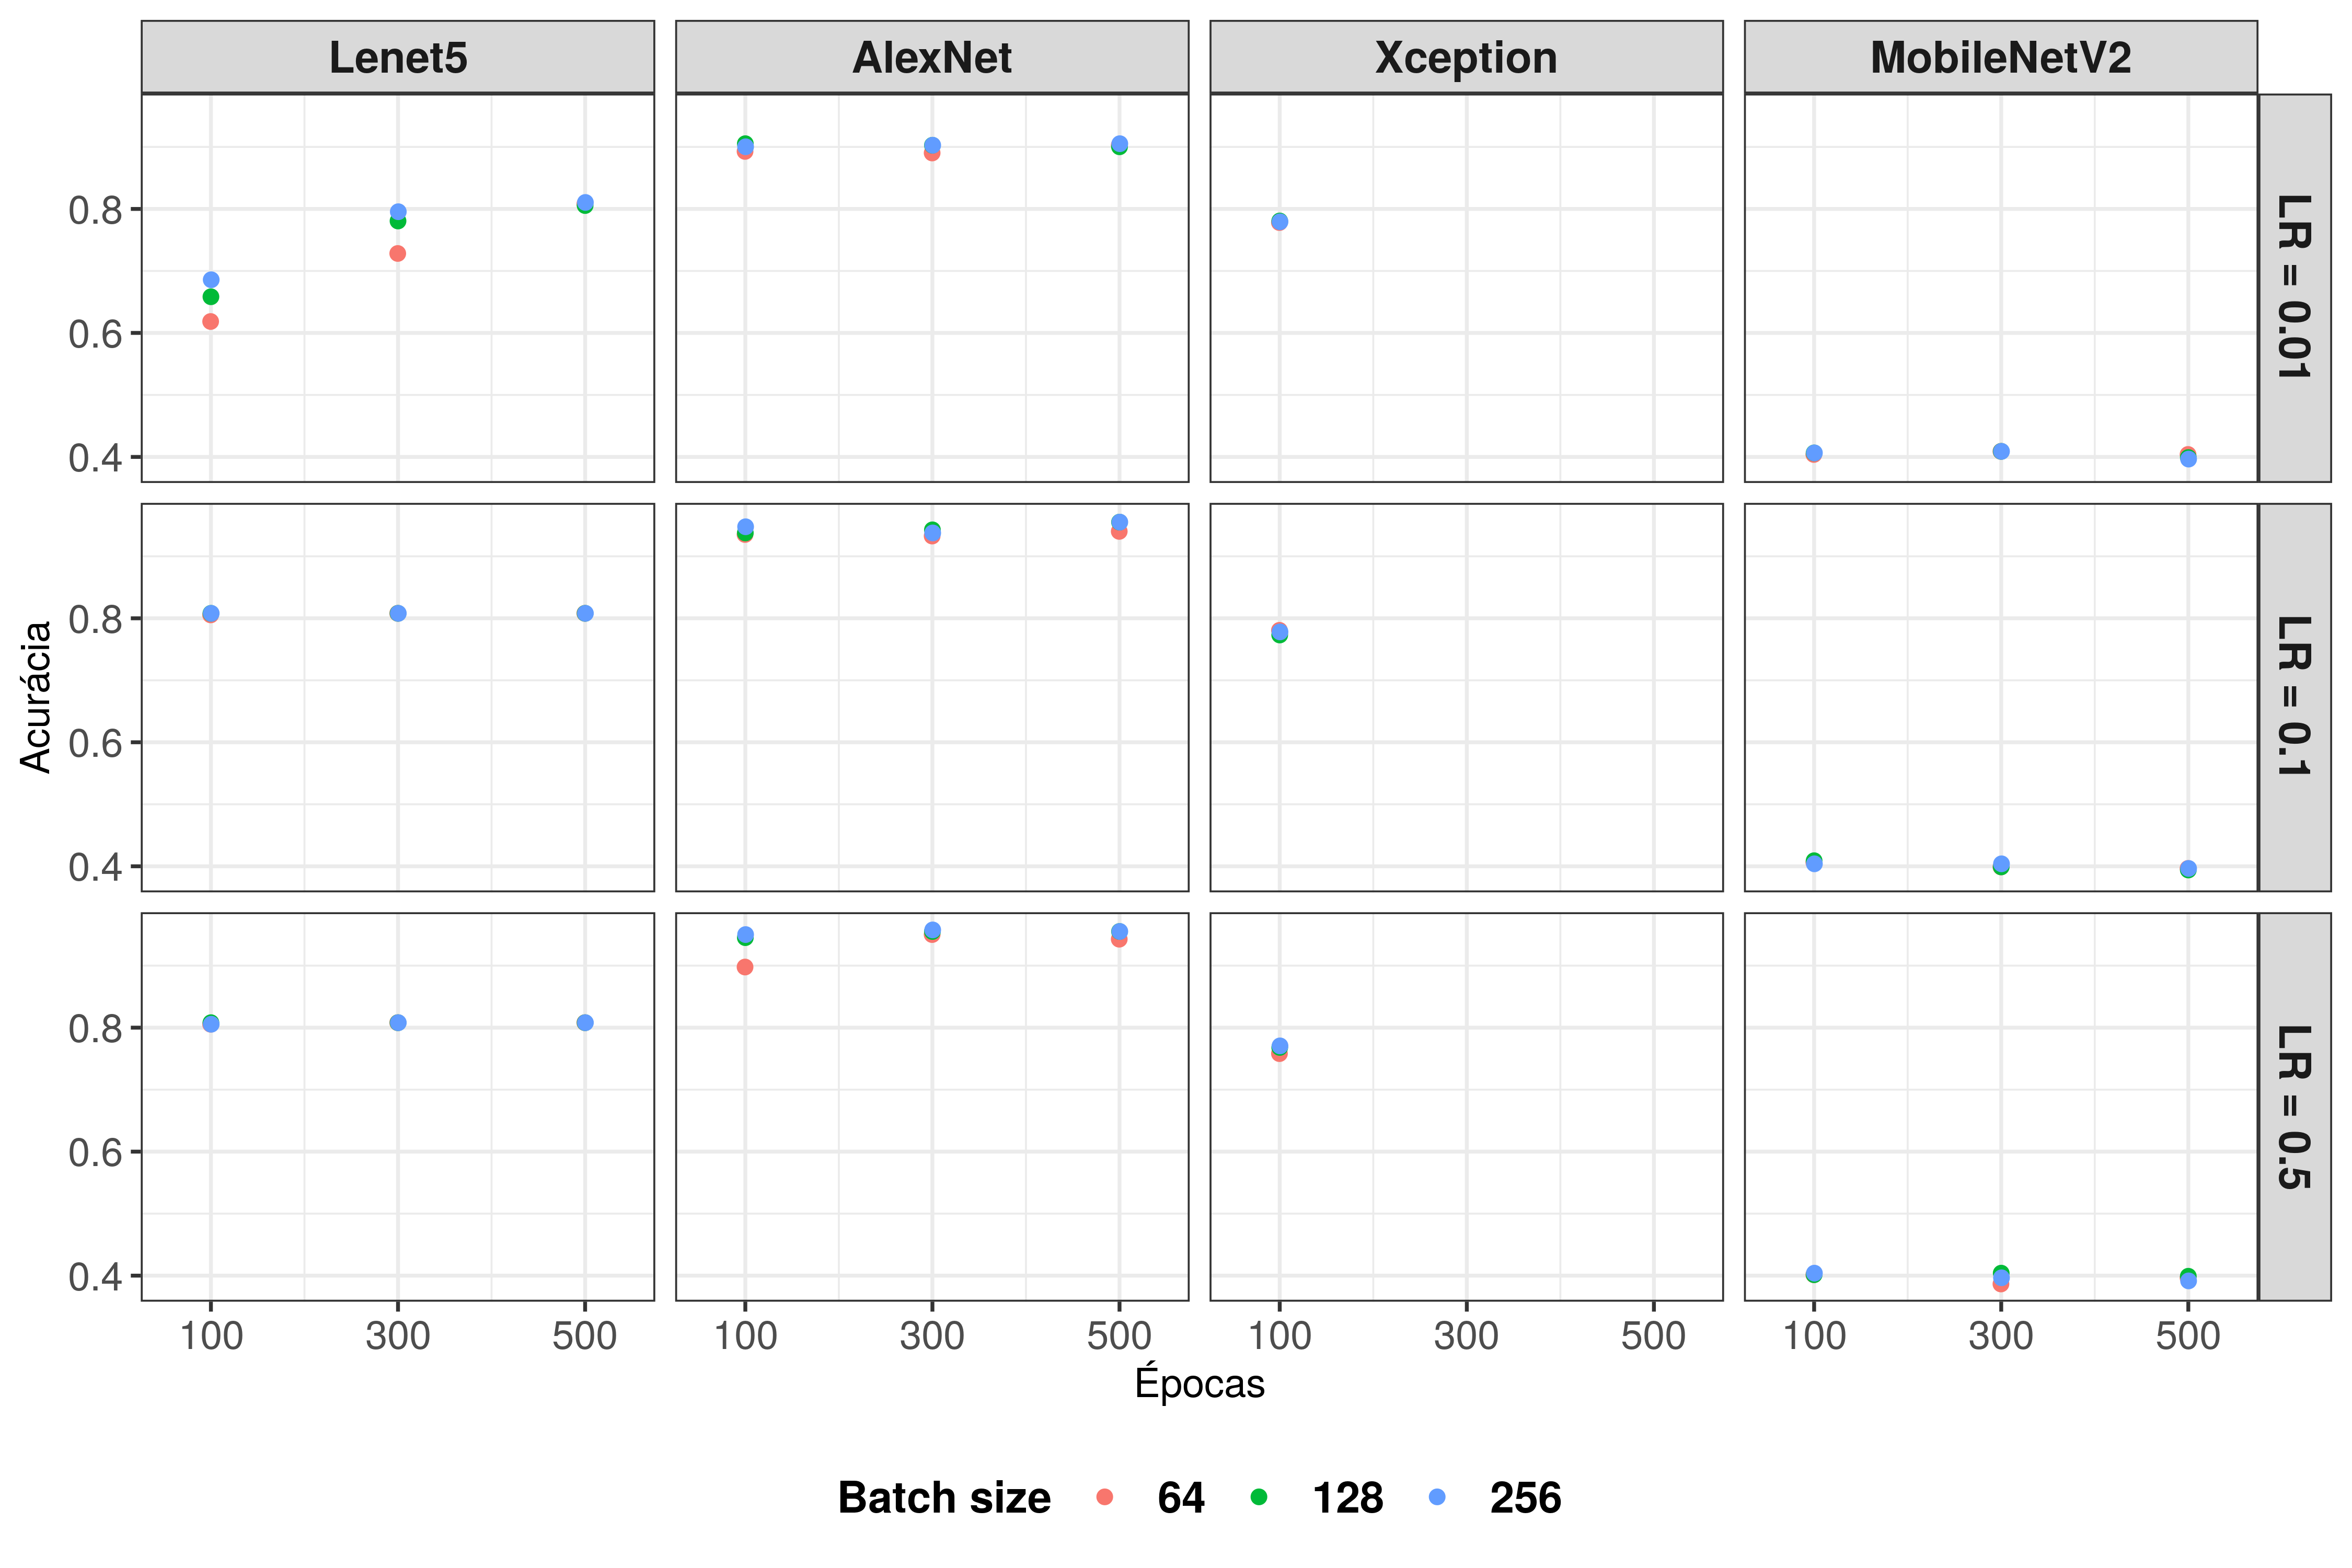
\includegraphics[width=1.6\textwidth]{/home/lacf14/machine_learning_ufpr/lab01/Analise/fig.png}
\caption{F1-score para cada combinação do experimento.}
\end{figure}
\end{landscape}

\chapter{Considerações finais}
\label{cap:conclusao}

% ----------------------------------------------------------------------
% CAPÍTULO 5 - CONCLUSÃO
% ----------------------------------------------------------------------

Os resultados mostraram que os melhores modelos eram aqueles com número reduzido de vizinhos, com distância Manhattan ou Euclidean e vetor de características vindos de imagens 20x20. Deste modo, não foi observado um ganho substancial ao aumentar-se o número de vizinhos ou o tamanho do vetor de características. As distâncias Manhattan ou Euclidean apresentaram resultados bastante similares e igualmente satisfatórios sendo que, em geral, opta-se pela distância Euclidean. Algo esperado e confirmado pelo experimento foi um desempenho similar entre diferentes algoritmos mostando que, para esse caso, a escolha pode ser simplesmente o mais rápido.

O experimento da forma que foi realizado apresenta algumas restrições: os resultados mostram que entre 1 e 5 vizinhos, a melhor performance é apresentada com apelas 1. Contudo em um experimento melhor delineado poderia ser investigado qual o melhor número de vizinhos testando uma quantidade maior de possibilidades, provavelmente seria um valor entre 1 e 5. 

Como outra restrição pode-se citar o tamanho do vetor de características. Foram testados 5 tamanhos, todos quadrados, em que o melhor foi aquele de tamanho 20x20. Os resultados mostraram em algum momento não faz mais diferença o acrécimo de características ao vetor de entrada, sendo que, provavelmente um vetor entre 100 e 400 características é bastante razoável.

Inicialmente havia interesse em testar também como se saía a distância de Mahalanobis, contudo esta apresentou problemas e foi abandonada no começo dos experimentos. 

Quanto aos algoritmos, não foi constatada uma diferença grande de desempenho entre as possibilidades, levando a crer que a escolha do mais rápido não traria prejuízos. Uma melhora neste experimento pode ser computar o tempo de execução nos cenários a fim concluir qual o mais rápido.

Por fim, vale ressaltar que esta análise foi meramente exploratória. Uma possibilidade seria, para cada cenário, gerar réplicas variando o conjunto de dados e analisar os resultados do experimento utilizando alguma metodologia estatística que permita estimar o efeito de cada fator sobre as métricas de qualidade de ajuste, tal como modelos de regressão.

% ---
\phantompart

% ---
% Conclusão
% ---

% ----------------------------------------------------------
% ELEMENTOS PÓS-TEXTUAIS
% ----------------------------------------------------------
\postextual

% ----------------------------------------------------------
% Referências bibliográficas
% ----------------------------------------------------------

%% Utilize este na elaboração do documento
\bibliography{refs}

%% Utilize este apenas ao final, quando não forem mais realizadas
%% alterações
% \begin{flushleft}
%   \small
% \renewcommand\refname{}
% \vspace*{-1.5cm}
% \input{01-tcc_corrigido.bbl}
% \end{flushleft}

% ----------------------------------------------------------
% Apêndices
% ----------------------------------------------------------

% ---
% Inicia os apêndices
% ---
% \begin{apendicesenv}

% Imprime uma página indicando o início dos apêndices
% \partapendices

% \chapter{Programas R}
% \label{capA:codigostcc}

% \end{apendicesenv}
% ---

% ----------------------------------------------------------
% Anexos
% ----------------------------------------------------------

%% % ---
%% % Inicia os anexos
%% % ---
%% \begin{anexosenv}
%% % Imprime uma página indicando o início dos anexos
%% \partanexos
%% \chapter{Lipsum}
%% \lipsum[30]
%% \end{anexosenv}

%---------------------------------------------------------------------
% INDICE REMISSIVO
%---------------------------------------------------------------------
% \phantompart
% \printindex
%---------------------------------------------------------------------

\end{document}
